\section{Optimization}
\label{sec:optimization}

This section presents the formulation of an optimization problem which yields controller parameters for the three domain gait of interest. The objective function of this optimization is a least squares fit of controller outputs to corresponding outputs computed on human locomotion data. More novel to this paper, however, is the construction of equality and inequality constraints that--when satisfied--yield periodic, three-domain walking. Previous results using partial hybrid zero dynamics are leveraged.  \textit{Motion Transitions} \cite{PHA2013} are used to compute the controller parameters for full actuation, $\alpha_{fa}$, and under actuation, $\alpha_{ua}$. State reconstruction on a partial hybrid zero dynamics surface \cite{WGK03} is used to compute various physical constraints on the controllers, e.g. torque and reaction force constraints.


\newsec{Partial Hybrid Zero Dynamics.}
Previous methods introduce the notion of \textit{partial hybrid zero dynamics} surface
\begin{align}
\label{PZD}
\mathcal{PZ}_{v,\alpha} = \{(q,\dot{q}) \in Q : y_{2}(q) = \mathbf{0}, \dot{y}_{2}(q,\dot{q}) = \mathbf{0}\}
\end{align}
which has properties that are useful for obtaining controllers for periodic walking, as described in the proceeding sections. In particular, on this surface, a low dimensional representation of the system is obtained by defining the zero dynamics coordinates for $v \in \{oa,fa\}$,
\begin{align}
\xi_{v,1} = \delta p_{hip}(q), \hspace{3mm}
\xi_{v,2} = c_{v}\dot{q}
\end{align}
The usefulness of this low dimensional representation will be demonstrated in the next section.

\newsec{Inverse Kinematics.} We use the method found in \cite{ACP:HSCC12}, to compute a point $\vartheta(\alpha_{oa}) \in Q_{r}$ on the guard from the underactuated phase to the double support phase, $S_{ua \to oa}$. We use the fact that on a partial hybrid zero dynamics surface $y^{a}_{2,v} = y^{d}_{2,v}$ and on $S_{ua \to oa}$, both the stance heel and the nonstance toe must be on the ground. The point is obtained by solving
\begin{eqnarray}
\label{eq:inverse}
\vartheta(\alpha_{oa}) = q \hspace{3mm} s.t. \hspace{5cm} \nonumber\\
\left[ \begin{array}{c}
y^{a}_{oa,2}(q) - y^{d}_{oa,2} (0,\alpha_{oa}) \\
h_{oa}(q)
\end{array}
\right] =
\left[ \begin{array}{c}
\zm_4 \\
0
\end{array}
\right],
\end{eqnarray}
where $\tau_{\alpha_{oa}} = 0$ at the beginning of the over actuated domain. Using $\vartheta(\alpha_{oa})$, we can explicitly solve for a point $(\vartheta, \dot{\vartheta}) \in \mathcal{PZ}_{\alpha_{oa}} \cap S_{oa}$.
%\textit{zero dynamics manifold}:
%\begin{align}
% \nonumber
%\ZeroDynamics_{\indexbyvertex{\param}} = \{(\q,\dq) \in \ConfigurationSpace :  \hspace{1mm} &\yone(\q,\dq) = 0, \\&
%\ytwo(\q) = \mathbf{0}, \ydottwo(\q,\dq) = \mathbf{0}\}
%\label{eq:ZD}
%\end{align}
%where $\yone(\q,\dq)$ and $\ytwo(\q,\dq)$ are a set of relative degree one and two outputs. The following is a Partial Zero Dynamics Surface
%\begin{align}
%\label{PZD}
%\PartialZeroDynamics_{\indexbyvertex{\param}} = \{(\q,\dq) \in \ConfigurationSpace : \ytwo(\q) = \mathbf{0}, \ydottwo(\q,\dq) = \mathbf{0}\}
%\end{align}
%This motivates the notion of a \textit{partial hybrid zero dynamics} on a cycle:
%\begin{align}
%\label{PZD}
%\forall \hspace{1mm} \edge \in \EdgeSet, \hspace{3mm} \indexbyedge{\resetmap} ( \indexbyedge{\guard} \cap \PartialZeroDynamics_{\param_\sore} ) \subset \PartialZeroDynamics_{\param_\tare}
%\end{align}

\newsec{PHZD State Reconstruction.}\label{sec:reconstruction} As claimed in \cite{ACP:HSCC12}, states on a partial hybrid zero dynamics surface can be obtained as functions of the linearized position of the hip. For $v \in \{V_{oa},V_{fa}\}$, the states of the system can obtained through PHZD reconstruction. It follows that by defining,
\begin{align}
\Phi(\xi_{v,1}) = 
\begin{bmatrix}
c_{v} \\
H_{v}
\end{bmatrix}^{-1}
\begin{bmatrix}
\xi_{v,1} \\
y^{d}_{v,2}
\end{bmatrix}
, \\
\Psi(\xi_{v,1}) = 
\begin{bmatrix}
c_{v} \\
H_{v}
\end{bmatrix}^{-1}
\begin{bmatrix}
1 \\
\frac{\partial y^{d}_{v,2}}{\partial \xi_{v,1}}
\end{bmatrix} \nonumber
\end{align}
the point $(\q, \dq) \in \mathcal{PZ}_{\param_{\vertex}}$ is found by $q  = \Phi(\xi_{v,1})$ and $\dq  = \dqreconstruction(\xi_{v,1})\xi_{v,2}$. The next section will show how motion transitions are used to compute controller parameters $\alpha_{fa}$ and $\alpha_{ua}$ in closed form.
\begin{comment}
Furthermore, this method can be used to compute states at \textit{any} value of $\xi_{1,\vertex}$;  in the proceeding sections we take advantage of this fact to specify values of $\xi_{1,\vertex}$ at 
which to transition from one domain to another. Let $\beta_1$ be a \textit{transition point} from 
the over actuated domain to the fully actuated domain, such that $(\qreconstruction(\beta_1)
,\dqreconstruction(\beta_1)) \in \guard_{oa \to fa}$ and likewise, let $\beta_2$ be a transition 
point from the fully actuated domain to the under actuated domain, such that $(\qreconstruction
(\beta_2),\dqreconstruction(\beta_2)) \in \guard_{fa \to ua}$.
\end{comment}

\newsec{Motion Transitions.} It was shown in \cite{PHA2013} that we can connect any two PHZD surfaces together with the ECWF to ensure that partial hybrid zero dynamics is maintained, i.e. there is a closed form expression for parameters of the ECWF that yield a PHZD surface connecting two other PHZD surfaces. Let $(\q_{\sore}, \dq_{\sore}) \in \mathcal{PZ}_{\param_{\sore}}$ and $(\q_{\tare}, \dq_{\tare}) \in \mathcal{PZ}_{\param_{{\tare}}}$ be points in two partial zero dynamics surfaces.
Denoting a set of controller parameters $\alpha$ for a set of ECWF's, leveraging the fact that the ECWF is linear in some of the controller parameters, it can be written as,
\begin{align}
\hspace{-2mm} y_{ecwf}(\alpha^{i},\tau) = Y_{ecwf}(\alpha^{i}_{2},\alpha^{i}_{4},\alpha^{i}_{6},\tau(\xi_{1},v_{hip},d))
\begin{bmatrix}
\alpha^{i}_{1} \\
\alpha^{i}_{3} \\
\alpha^{i}_{5} \\
\alpha^{i}_{7}
\end{bmatrix}
\end{align}
where,
\begin{align}
& Y_{ecwf}(\alpha^{i}_{2},\alpha^{i}_{4},\alpha^{i}_{6},\tau(q)) = \\
& \begin{bmatrix}
e^{-\alpha^{i}_{4}\tau(\xi_{1},v_{hip},d})cos(\alpha^{i}_{2}\tau(\xi_{1},v_{hip},d)) \\
e^{-\alpha^{i}_{4}\tau(\xi_{1},v_{hip},d})sin(\alpha^{i}_{2}\tau(\xi_{1},v_{hip},d)) \\
cos(\alpha^{i}_{6}\tau(\xi_{1},v_{hip},d))+\frac{2*\alpha^{i}_{4}\alpha^{i}_{6}}{(\alpha^{i}_{2})^{2}
+(\alpha^{i}_{4})^{2}-(\alpha^{i}_{6})^{2}} \\
1
\end{bmatrix}^{T} \nonumber
\end{align}
Using the states at the points to be connected to define,
\begin{align}
& y^{0}_{i,2} = y_{ecwf}(\tau(\xi_{1},v_{hip},d_{sor})\alpha^{i}) \\
& \dot{y}^{0}_{i,2} = \frac{d}{d\xi_{1}}y_{ecwf}(\tau(\xi_{1},v_{hip},d_{sor}),\alpha^{i})\Big|_{\xi_{1}=\xi^{0}_{1}} \\
& y^{f}_{i,2} = y_{ecwf}(\tau(\xi_{1},v_{hip},d_{tar}),\alpha^{i}) \\
& \dot{y}^{f}_{i,2} = \frac{d}{d\xi_{1}}y_{ecwf}(\tau(\xi_{1},v_{hip},d_{tar}),\alpha^{i})\Big|_{\xi_{1}=\xi^{f}_{1}},
\end{align}
where $\xi^{0}_{1}$ is the position of the hip at $q = q_{sor(e)}$ and $\xi^{f}_{1}$ the position of the hip at $q = q_{tar(e)}$, the controller parameters $\alpha_{1},\alpha_{3},\alpha_{5}$, and $\alpha_{7}$ that connect the source and target domains can be solved for,
\begin{align}
\begin{bmatrix}
\alpha^{i}_{1} \\
\alpha^{i}_{3} \\
\alpha^{i}_{5} \\
\alpha^{i}_{7}
\end{bmatrix}
=
\mathbb{Y}^{-1}
\begin{bmatrix}
y^{0}_{i,2} \\
\dot{y}^{0}_{i,2} \\
y^{f}_{i,2} \\
\dot{y}^{f}_{i,2}
\end{bmatrix}
\end{align}
where,
\begin{align}
 \mathbb{Y} = 
 \begin{bmatrix}
  Y_{ecwf}(\xi_{1},v_{hip},d_{sor},\alpha^{i}_{2},\alpha^{i}_{4},\alpha^{i}_{6}) \\
  \frac{d}{d\xi_{1}} Y_{ecwf}(\xi_{1},v_{hip},d_{sor},\alpha^{i}_{2},\alpha^{i}_{4},\alpha^{i}_{6})\Big|_{\xi_{1}=\xi^{0}_{1}} \\
  Y_{ecwf}(\xi_{1},v_{hip},d_{tar},\alpha^{i}_{2},\alpha^{i}_{4},\alpha^{i}_{6}) \\
  \frac{d}{d\xi_{1}} Y_{ecwf}(\xi_{1},v_{hip},d_{tar},\alpha^{i}_{2},\alpha^{i}_{4},\alpha^{i}_{6})\Big|_{\xi_{1}=\xi^{f}_{1}}
 \end{bmatrix}.
\end{align}
Note that the motion transition solves for $\alpha_{1},\alpha_{3},\alpha_{5}$, and $\alpha_{7}$, leaving $\alpha_{2},\alpha_{4}$ and $\alpha_{6}$ to be freely chosen as long as the chosen values satisfy $(\alpha^{i}_{2})^{2}+(\alpha^{i}_{4})^{2}-(\alpha^{i}_{6})^{2} \neq 0$ to prevent division 
by zero. For the purposes of this paper, the points $(q_{sor},\dot{q}_{sor})$ and $(q_{tar},\dot{q}_{tar})$ are 
obtained via the PHZD reconstruction at $((q,\dot{q}) \in \mathcal{PZ}_{oa}) \cap S_{oa \rightarrow fa}$ and $((q,\dot{q}) \in \mathcal{PZ}_{fa}) \cap S_{fa \rightarrow ua}$ to connect the outputs to the target $(\vartheta(\alpha_{oa}),\dot{\vartheta}(\alpha_{oa}))$ resulting in the controller parameters $\alpha_{fa}$ and $\alpha_{ua}$.
\begin{figure}[t!]
\centering
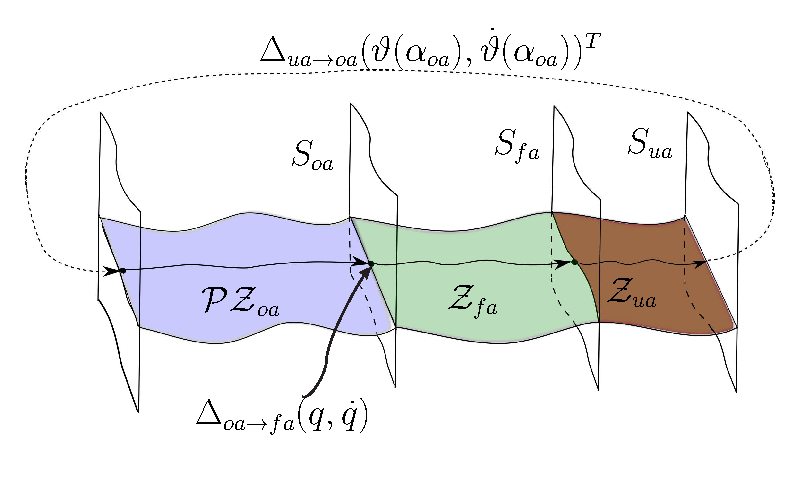
\includegraphics[scale=0.55]{figures/PZD_Surfaces_ICRA-crop.pdf}
% \hspace{-10mm}
\caption{Geometry of the close loop obtained using motion transitions.}
\label{fig:PZD_Surfaces}
% \vspace{50mm}
\end{figure}

\newsec{Human-Inspired Optimization.}
This section presents an optimization that yields controller parameters defining outputs that yield periodic, 3-domain walking. The key objective of the optimization is to find controller parameters defining referrence trajectories for each domain that minimize the least squares fit of these outputs to human walking data corresponding to the same outputs (see \cite{ZYA2012,YPA12} for the mathematical representation of this objective function).
%  From a subjects walking data, discrete times $t^{H}[k]$ and discrete values for the human output data, $y^{H}_{i,v}[k]$, for $i \in O_{v}$ where $O_{v}$ are indexing sets for the outputs in each domain $v \in V$. For clarity, the final discrete point in each domain will be denoted as $k_{v}$. For example, the last discrete time for the fully actuated domain will be referred to as $t[k_{fa}]$. With this in mind, the objective function for the human 
% inspired optimization is expressed mathematically as,
% \begin{align}
% \label{eq:cost}
% \hspace{-6mm} \mathrm{Cost_{HD}}(\alpha_{v}) = 
%  \sum\limits_{i \in O_{oa}}\sum\limits_{k = 1}^{k_{oa}}(y^{H}_{i}[k] - y^{d}_{oa,i}(t^{H}[k],\alpha_{oa,i}))^{2} \\ + 
%  \sum\limits_{j \in O_{fa}}\sum\limits_{k = k_{oa}}^{k_{fa}}(y^{H}_{j}[k] - y^{d}_{fa,j}(t^{H}[k],\alpha_{fa,j}))^{2} \hspace{-3mm} \nonumber \\ +
%  \sum\limits_{m \in O_{ua}}\sum\limits_{k = k_{fa}}^{k_{ua}}(y^{H}_{m}[k] - y^{d}_{ua,m}(t^{H}[k],\alpha_{ua,m}))^{2} \hspace{-6mm} \nonumber 
% \end{align}
% Minimizing this cost means finding controller parameters that are as close to the human data as possible thus resulting in humanlike locomotion.

\newsec{Force Based Constraints.} To compute force based constraints, the contact forces and moments at each contact point are computed using standard methods (see \cite{GCAS10}). The three contact conditions encountered in the 3 domain walking considered include: $c_{oa} = \{sh, nst\}$, $c_{fa} = \{st, sh\}$, and $c_{ua} = st$. Furthermore, a wrench containing contact forces and moments will exist for each point in contact, i.e. $F_{v,i} = (F^{x}_{v,i},F^{z}_{v,i},M^{y}_{v,i})$ for $i \in c_{v}$. A constraint is needed to ensure the vertical component of the contact force for each contact in each domain is greater than or equal to zero,
\begin{align}
min(F^{z}_{v,i}) \geq 0 \tag{C1}
\end{align}
Additionally, in order to prevent the feet from slipping, the following constraint must be satisfied:
\begin{align}
|F^{x}_{v,i}| < \frac{\mu}{\sqrt{2}} F^{z}_{v,i} \hspace{-3mm} \tag{C2-C6}
\end{align}
where $\mu$ is the friction coefficient of the walking surface. Also note that there will be a friction constraint 
for each contact point in each domains, leading to five friction constraints in total.

\newsec{Zero Dynamics Constraints.} The partial hybrid zero dynamics surface defined in \eqref{PZD} is defined for the continuous dynamics only, meaning any disturbances will lead to the system being thrown from this surface. It is for this that constraints are needed to ensure the zero dynamics surfaces are invariant to the 
impacts. To construct this constraint it is first necessary to define the \emph{full zero dynamics surface},
\begin{align}
\mathcal{Z}_{v} = \{(q,\dot{q}) \in Q : y_{v}(q) = \mathbf{0}, \dot{y}_{v}(q,\dot{q}) = \mathbf{0}\}
\end{align}
where $y_{v}(q)$ contains all relative degree one and/or two outputs in the domain $v$. With this, 
a constraint can be formulated to ensure the transition from full actuation to over actuation is 
invariant to the impact at heel strike. This constraint is expressed mathematically as,
\begin{align}
\Delta_{ua \rightarrow oa}(S_{ua} \cap \mathcal{Z}_{ua}) \subset \mathcal{PZ}_{oa} \tag{C7}
\end{align}
where $\Delta_{ua \rightarrow oa}$ represents the application of the impact map.

\newsec{Optimization Formulation.} With the controllers and constraints defined, the final form of the human inspired, 3-domain optimization becomes,
\begin{align}
\label{eq:OptimizationFinal}
 (\alpha^{*}_{v},d^{*}_{fa},d ^{*}_{ua}) =  \underset{\alpha_{oa},d_{fa},d_{ua}\in \mathbb{R}^{27}}{argmin}  \mathrm{Cost_{HD}}(\alpha_{v}) \\ \vspace{1mm}
 s.t. \hspace{3mm} (C1,C2,...,C7) \hspace{3mm} \nonumber
\end{align}
It is important to recall that $\alpha_{fa}$ and $\alpha_{ua}$ are solved for in closed form within the optimization 
using motion transitions, thus initial guesses for these parameters are not needed.
\begin{comment}
 These are the conditions needed to solve for controller parameters $\alpha$ corresponding to a motion transition from $(\q^{\sore}, \dq^{\sore})$ to  $(\q^{\tare}, \dq^{\tare})$:
\begin{align}
\label{eq:transitionsource}
  y^d_{2,{\tare}}(\timeparameterization_{\tare}(\q^{\sore}),\paramtransition_i) &= y^d_{2,{\sore}}(\timeparameterization_{\sore}(\q^{\sore}),\param_{\sore,i}) \nonumber\\
 {\dot y}^d_{2,{\tare}}(\timeparameterization_{\tare}(\q^{\sore}),\paramtransition_i) &={\dot y}^d_{2,{\sore}}(\timeparameterization_{\sore}(\q^{\sore}),\param_{\sore,i})\nonumber\\
 y^d_{2,{\tare}}(\timeparameterization_{\tare}(\q^{\tare}),\paramtransition_i) &= y^d_{2,{\tare}}(\timeparameterization_{\tare}(\q^{\tare}),\param_{\tare,i}) \nonumber\\
 {\dot y}^d_{2,{\tare}}(\timeparameterization_{\tare}(\q^{\tare}),\paramtransition_i) &= {\dot y}^d_{2,{\tare}}(\timeparameterization_{\tare}(\q^{\tare}),\param_{\tare,i}) 
\end{align}
for all $i \in \OutputSet_{\tare}$. 
\begin{myexample}
In this work, we construct two motion transitions $\alpha_{fa}$ and $\alpha_{ua}$. Naturally, the first transition,  $\alpha_{fa}$,  occurs at the first \textit{transition point}, $\beta_1$, i.e. when $ \timeparameterization_{\param_{oa}}(\q) = \beta_1$. The first motion transition connects $\resetmap_{oa \to fa} ( \guard_{oa \to fa} \cap \PartialZeroDynamics_{\param_{oa}} )$ to $(\thetaalpha, \thetaalphadot)$.  Likewise, the second transition , $\alpha_{ua}$, occurs at the second transition point, $\beta_2$, i.e. when $ \timeparameterization_{\param_{fa}}(\q) = \beta_2$. The second motion transition connects $\resetmap_{fa \to ua} ( \guard_{fa \to ua} \cap \PartialZeroDynamics_{\param_{fa}} )$ with $(\thetaalpha, \thetaalphadot)$.
\end{myexample}

\begin{comment}
%HERE IS AN ALTERNATE EXPRESSION FOR A MOTION TRANSITIONS (FAIL)
%\begin{mydefinition}
%Controller parameters $\alpha$ of the extended canonical walking function are said to form a \textit{Motion Transition} from $x_1 = (\q_1^T,\dq_1^T)^T$ to  $x_2 = (\q_2^T,\dq_2^T)^T $ REF if
%\begin{align}
%\exists \alpha \st &  \:\: \nonumber \\
% (\q_1^T,\dq_1^T)^T  &\in \PartialZeroDynamics_{\alpha} \\
% (\q_2^T,\dq_2^T)^T  &\in \PartialZeroDynamics_{\alpha}
%\end{align}
%\end{mydefinition}


%
%In particular, the velocities, $\thetaalphadot$ are obtained through
%\begin{align}
%\label{eq:inverse_dot}
%\thetaalphadot = \left[ \begin{array}{c} \indexbyvertex{\dyonedq} \\ \indexbyvertex{\dytwodq} \end{array} \right]^{-1} \left( \begin{array}{c} \vhip \\ \zm \end{array} \right).
%\end{align}




%\begin{align}
%\qreconstruction(\xi_{1,\vertex}) &= \left[ \begin{array}{c} \indexbyvertex{\dyonedq} \\ \indexbyvertex{\dytwodq} \end{array} \right]^{-1} \left( \begin{array}{c} \xi_{1,\vertex} \\ \ydtwo (\xi_{1,\vertex}) \end{array} \right)\\
%\dqreconstruction(\xi_{1,\vertex}) &= \left[ \begin{array}{c} \indexbyvertex{\dyonedq} \\ \indexbyvertex{\dytwodq} \end{array} \right]^{-1} \left( \begin{array}{c} 1 \\ \frac{\partial \ydtwo (\xi_{1,\vertex})}{\partial \xi_{1,\vertex}} \end{array} \right)
%\end{align}



%\newsec{Optimization Cost.}
%The objective function of this optimization is a least squares fit of controller outputs to corresponding outputs computed on human locomotion data, over all three domains. The controller parameters for the full actuation, $\indexbyfullactuation{\param}$, and the under actuation, $\indexbyunderactuation{\param}$, domains are obtained through motion transitions, specifically \eqref{eq:transitionsource} and \eqref{eq:transitiontarget}. The human data, with discrete times $t^H[k]$ and values for outputs, $y^H_i[k]$, is indexed by a set $K$, where $k \in \{1, \ldots, K\}$ represents indices for discrete data points, and $t^H[k] < t^H[k+1] \forall k \in K$. Let $K_{\beta_1}$ denote the time corresponding to a transition from $oa \to fa$ and $K_{\beta_2}$ denote the time corresponding to a transition from $fa \to ua$. For each relative degree two output, $i \in \OutputSet_v$ for a given domain, $\vertex \in \VertexSet$, the value of the output is denoted $y^d_i(t^H[k],\param_{v,i})$  . The total cost is the sum of the costs of each domain, which can be stated as follows
%\begin{align}
%\nonumber
%\costoa(\indexbydoublesupport{\param} ) =  \sum_{k = 1}^{K_{\beta_1}} \sum_{i \in \OutputSet_{oa}} \left( y^H_i[k] - y^d_i(t^H[k],\param_{oa,i}) \right)^2
%\end{align}
%\begin{align}
%\nonumber
%\costfa(\indexbydoublesupport{\param} ) =  \sum_{k = K_{\beta_1}}^{K_{\beta_2}} \sum_{i \in \OutputSet_{fa}} \left( y^H_i[k] - y^d_i(t^H[k],\alpha_{(fa,i)}(\param_{oa}) \right)^2
%\end{align}
%\begin{align}
%\nonumber
%\costua(\indexbydoublesupport{\param} ) =  \sum_{k = K_{\beta_2}}^{K} \sum_{i \in \OutputSet_{ua}} \left( y^H_i[k] - y^d_i(t^H[k],\alpha_{(ua,i)}(\param_{oa})  \right)^2
%\end{align}
%\begin{align}
%\label{eq:HDBC}
%\HDBC(\indexbydoublesupport{\param} ) =  \costoa(\indexbydoublesupport{\param} ) + \costfa(\indexbydoublesupport{\param} )+ \costua(\indexbydoublesupport{\param} )
%\end{align}
%which quantifies the similarity between the human and the robot outputs.



\newsec{Optimization Problem Statement.} The goal of \textit{human-inspired PHZD optimization} is to find parameters $\indexbydoublesupport{\param^*}$ that solve the following constrained optimization problem:
\begin{align}
\label{eq:PHZDopt}
\tag{HIO}
(\indexbydoublesupport{\param}^*, \beta^*) = \underset{(\indexbydoublesupport{\param}, \beta)  \in \Reals^{21} \times \Reals^{2} }{\operatorname{argmin}} &  \:\: \HDBC(\indexbydoublesupport{\param} )  \\
%\tag{C}
\st &  \:\: \nonumber \\
\label{eq:C1}
\tag{C1}
\resetmap_{fa \to oa} ( \guard_{fa \to oa} \cap \PartialZeroDynamics_{\alpha_{fa}(\param_{oa}, \beta)} ) &\subset \PartialZeroDynamics_{\param_{oa}} \\
\label{eq:C2}
\tag{C2}
\resetmap_{oa \to ua} ( \guard_{oa \to ua} \cap \PartialZeroDynamics_{\param_{oa}} ) &\subset \PartialZeroDynamics_{\alpha_{ua}(\param_{oa}, \beta)}  \\
\label{eq:C3}
\tag{C3}
\resetmap_{ua \to fa} ( \guard_{ua \to fa} \cap \PartialZeroDynamics_{\alpha_{ua}(\param_{oa}, \beta)} ) &\subset \PartialZeroDynamics_{\alpha_{fa}(\param_{oa}, \beta)} \\
\label{eq:C4}
\tag{C4}
(\qreconstruction (\beta_1), \dqreconstruction (\beta_1)) &\in \guard_{oa \to fa} \\
\label{eq:C5}
\tag{C5}
(\qreconstruction (\beta_2), \dqreconstruction (\beta_2)) &\in \guard_{fa \to ua} \\
\label{eq:C6}
\tag{C6}
\indexbydoublesupport{\ConstraintMatrix}(\qreconstruction (\xi_{1,oa}),\dqreconstruction (\xi_{1,oa}), \indexbydoublesupport{\control}) &\geq 0 \\
\label{eq:C7}
\tag{C7}
\indexbyfullactuation{\ConstraintMatrix}(\qreconstruction (\xi_{1,fa}),\dqreconstruction (\xi_{1,fa}), \indexbyfullactuation{\control}) &\geq 0 \\
\label{eq:C8}
\tag{C8}
\indexbyunderactuation{\ConstraintMatrix}(\qreconstruction (\xi_{1,ua}),\dqreconstruction (\xi_{1,ua}), \indexbyunderactuation{\control}) &\geq 0
\end{align}
where $\HDBC(\param_{oa})$ is essentially the same cost as the original human data based cost given in EQREF.; where here, the contribution to the cost in each domain is the least squares fit of human data to the desired values of each controller output. Note that the motion transitions, $\alpha_{fa}$ and $\alpha_{ua}$, are functions of both $\alpha$ and $\beta$ because 

\begin{algorithm}
\caption{Algorithm for obtaining controller parameters for a three-domain locomotion gait.}
%The optimization procedure follows:
\begin{itemize}[\setlabelwidth{Step 1}]
\item[Step 1)] Initialize values for the controller parameters, $\param_{oa}$, and the domain transition points, $\beta$.
\item[Step 2)] Solve the inverse kinematics problem, yielding $(\thetaalpha, \thetaalphadot)$-- the initial condition to the double support domain on the partial hybrid zero dynamics surface.
\item[Step 3)] Compute the state reconstruction for the double support domain and use this reconstruction to compute inequality constraints \eqref{eq:C6} on the domain of admissibility $\domain_{oa}$ for double support.
\item[Step 4)] Compute the state reconstruction at the first transition point, $\xi_{1,oa} = \beta_1$, and use this point to compute equality \eqref{eq:C4} constraints on the guard from double support to full actuation, $\guard_{oa \to fa}$.
\item[Step 5)] Compute parameters for the full actuation domain, $\alpha_{fa}$, that construct a motion transition EQREF from $(\qreconstruction (\beta_1),\dqreconstruction (\beta_1),\param_{fa}) \to (\thetaalpha, \thetaalphadot)$ .
\item[Step 6)] Compute the state reconstruction for the full actuation domain and use this reconstruction to compute inequality constraints \eqref{eq:C7} on the domain of admissibility $\domain_{fa}$ for full acutation.
\item[Step 7)] Compute the state reconstruction at the second transition point,  $\xi_{1,fa} = \beta_2$,  and use this point to compute equality \eqref{eq:C5} constraints on the guard from full actuation to under actuation, $\guard_{fa \to ua}$.
\item[Step 8)] Compute parameters for the under actuation domain, $\tilde{\alpha}_{ua}$, that construct a motion transition EQREF from $(\qreconstruction (\beta_2),\dqreconstruction (\beta_2),\param_{ua}) \to (\thetaalpha, \thetaalphadot)$.
\item[Step 9)] Integrate through the underactuated domain to compute inequality constraints \eqref{eq:C8} on the domain of admissibility $\domain_{ua}$ for under actuation.
\item[Step 10)] Compute $\HDBC(\param_{oa})$.
\item[Step 11)] Iterate the nonlinear constrained optimization problem one step, \ref{eq:PHZDopt}, to obtain values for $\param_{oa}$ and $\beta$.
\item[Step 12)] Repeat the iteration until local minimum reached, yielding optimal controller parameters, $\param_{oa}^*$, and domain transition points, $\beta^*$.
\end{itemize}
\end{algorithm}
\end{comment}
